\begin{flushleft}

Da zuvor noch keine Vorerfahrungen zum Erstellen von React-Apps bestand, erfolgte hier erst eine Einarbeitung in diverse Grundlagen und Funktionalitäten in  React.
React ist ein Javascript Framework zum Entwickeln von Webseiten und Webanwendungen.
Statt einfachen statischen HTML-Seiten wird hier mit sogenannten Komponenten gearbeitet, die mehrfach verwendet werden können.
Ebenso können mit States und Hooks reaktive Single-Page-Applications erstellt werden, die ein re-rendern der jeweiligen Komponenten erlauben, ohne ein Neuladen der ganzen Seite.
Weitere Pakete und Bibliotheken können mit dem Paketmanager npm ebenfalls jederzeit nachinstalliert werden.

So gibt es auch die \textit{roslibjs} Bibliothek im npm-Paketstore.
Installation und Importierung in das aktuelle Projekt wird in [\ref{frontend_install}] ausführlicher Beschrieben.
% \begin{lstlisting}[language=bash]
%     npm install roslib 
% \end{lstlisting}

% wird diese dem Projekt hinzugefügt und kann in folgender Weise inkludiert werden:

% \begin{lstlisting}
%     import ROSLIB from 'roslib';
% \end{lstlisting}

Bezüglich der Architektur, bzw. dem Aufbau der Website, haben wir uns an die standardmäßige Vorgehensweise in React gehalten, in dem man die Seite in Komponenten aufteilt und diese so an mehreren Stellen wieder verwenden kann. Dafür haben wir einen extra Verzeichnis \textit{/components} im \textit{/src} Verzeichnis angelegt, sowie eines mit \textit{/pages} für die jeweiligen Seiten. Diese werden in der \textit{App.js} Datei mit dem \textit{react-router-dom} Paket geroutet.


Wir haben uns für eine linksbündige Navigationsleiste entschieden, da diese mehr zu einem Dashboard und einer Konfigurationsseite passt. Auch hier wurde im ersten Moment nicht viel Wert auf ein besonders ausgefallenes Design gelegt. Eine schwarze Navigationsleiste mit einem aufklappbarem Burgermenü war hier für uns ausreichend. 

\hypertarget{rosboard-target}{Für} den generellen Aufbau und dem Design der Website hatten wir uns im Vorfeld schon Gedanken gemacht, so war es uns auf jeden Fall wichtig eine Übersichtseite mit allen Topics zu haben und von diesen die Inhalte auslesen zu können.
Im laufe der Wochen hatten wir ein Gespräch mit Benjamin Stähle aus dem RoboLab an der RWU, wir erzählten ihm von unserem Vorhaben und er zeigte uns ein ROS-Webdashboard namens \textit{rosboard}.
Diese Plattform hatte quasi die Funktionen, die wir für unsere Webanwendung auch geplant hatten.
Zu diesem Zeitpunkt überlegten wir uns, ob wir von nun an diese verwenden, oder unsere eigene Webanwendung programmierten.
Natürlich hätte es hier schon alle unsere gewünschten Funktionen zur Verfügung gehabt, allerdings entschieden wir uns dafür, einmal diesen Prozess von Grund auf selber zu entwickeln und unsere eigene ROS-Webanwendung zu erstellen.
Wir wollten uns aber vom Design und der Vorgehensweise trotzdem an der vorgestellten Anwendung von \textit{rosboard} orientieren.
Ebenso unterscheidet diese sich auch von der Implementierung, da diese auf ganze andere Bibliotheken basiert.
\\

\vspace{0.5cm}
Um nun die Vorteile von React in unserer Anwendung sinnvoll zu nutzen, unterteilten wir das Connection-Handling, Publishen, Subscriben oder auch beispielsweise die Auflistung der aktuellen Topics, in eigene Komponenten auf.
So konnten wir mit Hilfe von useState-Hooks und useContext-Hooks, eine Singlepage-Application bauen, die mehrere Verbindungen zu ROS-Instanzen verwalten kann.
Für jede offene Verbindung wird ein neues ROSLIB-Objekt angelegt und in ein Array gespeichert.
So kann für jedes dieser Objekte eine neue eigene Unterseite erstellt werden, um mit dem ROS-Topics zu interagieren. Diese werden ebenso im Dashboard in einer Tabelle ausgegeben (siehe Abbildung \ref{fig:ros_conn}).

\begin{figure}[h!]
    \centering
    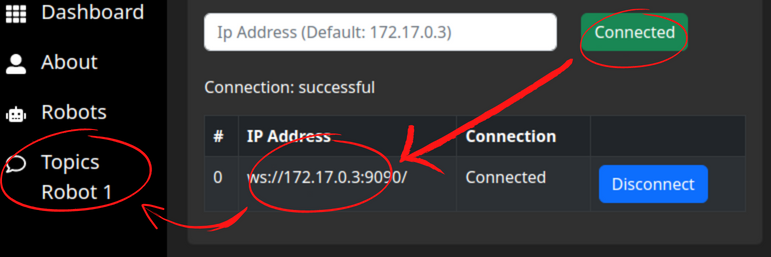
\includegraphics[width=0.8\textwidth]{imgs/web/ros_conn.png}
    \caption{Connection Handler mit Liste und automatischem Navigationspunk}
    \label{fig:ros_conn}%
\end{figure}
\end{flushleft}
    